% Appendix: supporting detail and case studies for Introspective Verification.
% All numbers are computed from the released dumps of our own runs (layerfeats.npz,
% pa15_full.npz, pa_4000_ml4096.npz) with the localization-F1 metric of the main text.
% Style: plain, direct; no em-dashes; minimal colons/quotes.

\section{Supporting detail}
\label{app:experiments}

This appendix collects supporting detail and two case studies. \Cref{app:layersweep} gives the full per layer probe numbers behind \Cref{fig:layersweep}, \Cref{app:calib} explains the scale specific median shift used only at 7B, and \Cref{app:omnimath} documents the OmniMATH ranking limit. The two case studies in \Cref{app:cases} show, on real ProcessBench cases, the complementary failures that the fusion of \Cref{sec:exp-7b} exploits. Unless stated otherwise the metric is ProcessBench localization F1 and every number is computed from our own score dumps.

\subsection{Per layer probe sweep}
\label{app:layersweep}

\Cref{fig:layersweep} plots the per layer probe separability of \Cref{tab:layersweep} as a curve against relative depth. We freeze the 7B backbone, take the last token hidden state of each step at eight candidate layers, fit a balanced logistic probe on step correctness, and report the step level AUC on a held out split of the training pool and the probe localization F1 on 140 held out cases. Both peak at about seventy percent of the depth and fall off toward the final layer and toward the middle of the network.

\begin{figure}[h]
  \centering
  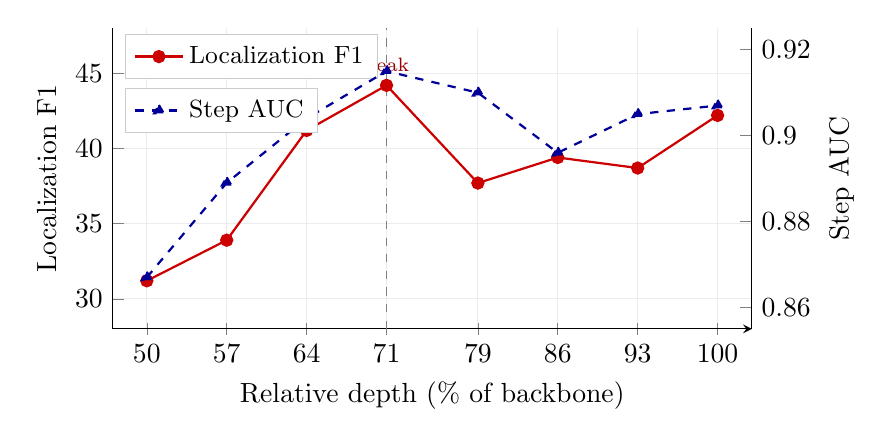
\begin{tikzpicture}
    \begin{axis}[
      width=0.80\linewidth, height=5.4cm,
      axis y line*=left, axis x line=bottom,
      xlabel={Relative depth (\% of backbone)}, ylabel={Localization F1},
      xmin=47, xmax=103, ymin=28, ymax=48,
      xtick={50,57,64,71,79,86,93,100},
      ytick={30,35,40,45},
      grid=major, grid style={gray!15},
      legend style={at={(0.02,0.98)}, anchor=north west, font=\small, draw=gray!40},
    ]
    \addplot[mark=*, thick, color=red!80!black] coordinates {(50,31.2)(57,33.9)(64,41.2)(71,44.2)(79,37.7)(86,39.4)(93,38.7)(100,42.2)};
    \addlegendentry{Localization F1}
    \draw[dashed, gray] (axis cs:71,28) -- (axis cs:71,48);
    \node[anchor=south, font=\scriptsize, red!60!black] at (axis cs:71,44.2) {peak};
    \end{axis}
    \begin{axis}[
      width=0.80\linewidth, height=5.4cm,
      axis y line*=right, axis x line=none,
      ylabel={Step AUC}, ymin=0.855, ymax=0.925,
      xmin=47, xmax=103, ytick={0.86,0.88,0.90,0.92},
      legend style={at={(0.02,0.80)}, anchor=north west, font=\small, draw=gray!40},
    ]
    \addplot[mark=triangle*, thick, dashed, color=blue!60!black] coordinates {(50,0.867)(57,0.889)(64,0.904)(71,0.915)(79,0.910)(86,0.896)(93,0.905)(100,0.907)};
    \addlegendentry{Step AUC}
    \end{axis}
  \end{tikzpicture}
  \caption{Per layer probe separability on the frozen 7B backbone (the curve behind \Cref{tab:layersweep}). Both the step level AUC (right axis) and the probe localization F1 (left axis) peak at about seventy percent of the depth and fall off toward the final layer at the right edge.}
  \label{fig:layersweep}
\end{figure}

\subsection{A calibration trick for the 7B fusion}
\label{app:calib}

The 7B fusion uses one small unsupervised trick, which we report for completeness rather than as part of the method. The 7B head assigns systematically different logit levels to different domains, so a single global decision threshold is misaligned per domain and is too strict on OlympiadBench in particular. Subtracting each domain's own median logit, which needs no labels, realigns the domains to a common threshold. This raises the standalone 7B head from 64.2 to 68.5 mean F1 and is what lets the honest fusion reach 77.4. The 1.5B head does not show this drift. Its per domain logit levels already sit near a common threshold, so the same shift adds nothing and slightly hurts, since on OmniMATH it removes useful spread. The difference is one of scale, the larger and more specialized backbone separates domains more strongly in its logit scale, so we apply the shift only at 7B.

\subsection{The OmniMATH ranking limit}
\label{app:omnimath}

OmniMATH is the proof heavy subset and the hardest for the cheap head. Its per step separability is the lowest of the four subsets, a step level AUC of 0.866 against 0.889 on GSM8K (\Cref{tab:perdomain}), but the sharper limit is localization on correct and on long solutions. The head has its lowest correct solution accuracy on OmniMATH, 57.7 percent, so it over flags correct proofs, and its highest wrong step rate, 44.3 percent, so when a proof is wrong it often marks the wrong step. Both effects grow with solution length (\Cref{fig:length,fig:errpos}). This is why the standalone head is weakest on OmniMATH in \Cref{tab:pb}, and why the fusion defers to the generative verifier there. We treat it as an honest limit of a single forward pass read on long free form proofs.

\section{Extended quantitative analysis}
\label{app:extended}

We analyze the head in more depth from the same score dumps. Unless noted the scale is 1.5B on the full benchmark, and the metric is localization F1 or step level AUC as defined in \Cref{sec:exp-setup}.

\subsection{Threshold sensitivity}
\label{app:thr}

The head returns a per step probability, and a single threshold turns it into a decision. \Cref{fig:thrsweep} sweeps this threshold per subset. GSM8K is nearly flat and peaks around 0.87, while the proof heavy subsets keep improving toward a stricter threshold, since the head over flags there and a higher bar removes false alarms. A single threshold tuned on a held out split, 0.92, is a compromise across subsets. This per subset disagreement in the best threshold is what the unsupervised per domain calibration of \Cref{app:calib} exploits at 7B.

\begin{figure}[h]
  \centering
  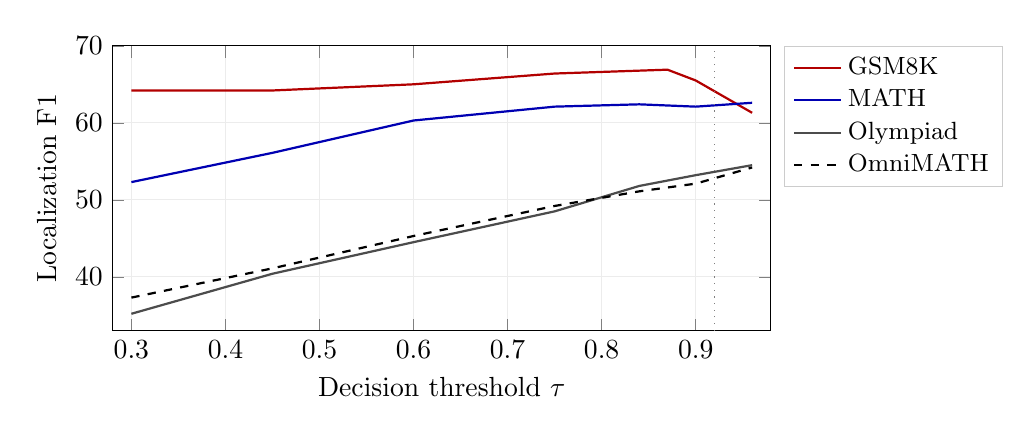
\begin{tikzpicture}
    \begin{axis}[width=0.82\linewidth, height=5.2cm, xlabel={Decision threshold $\tau$}, ylabel={Localization F1},
      xmin=0.28, xmax=0.98, ymin=33, ymax=70, grid=major, grid style={gray!15},
      legend style={at={(1.02,1)}, anchor=north west, font=\small, draw=gray!40}, legend cell align=left]
    \addplot[thick,color=red!70!black] coordinates {(0.3,64.2)(0.45,64.2)(0.6,65.0)(0.75,66.4)(0.87,66.9)(0.9,65.5)(0.96,61.3)};
    \addlegendentry{GSM8K}
    \addplot[thick,color=blue!70!black] coordinates {(0.3,52.3)(0.45,56.1)(0.6,60.3)(0.75,62.1)(0.84,62.4)(0.9,62.1)(0.96,62.6)};
    \addlegendentry{MATH}
    \addplot[thick,color=gray!60!black] coordinates {(0.3,35.2)(0.45,40.4)(0.6,44.5)(0.75,48.5)(0.84,51.8)(0.9,53.2)(0.96,54.5)};
    \addlegendentry{Olympiad}
    \addplot[thick,dashed,color=black] coordinates {(0.3,37.3)(0.45,41.1)(0.6,45.3)(0.75,49.2)(0.84,51.1)(0.9,52.1)(0.96,54.2)};
    \addlegendentry{OmniMATH}
    \draw[dotted,gray] (axis cs:0.92,33)--(axis cs:0.92,70);
    \end{axis}
  \end{tikzpicture}
  \caption{Localization F1 against the decision threshold for LVH-1.5B. GSM8K peaks early while the proof heavy subsets prefer a stricter threshold. The dotted line is the single held out tuned threshold.}
  \label{fig:thrsweep}
\end{figure}

\subsection{Calibration}
\label{app:calibration}

The head returns a probability, and \Cref{fig:calib} checks how well that probability matches the empirical error rate. It does not. The head is over confident, with an expected calibration error of 0.238, and steps to which it assigns a probability near one are in fact error steps only 41 percent of the time. This is why inference tunes a single threshold rather than reading the probability at 0.5, and it is consistent with the per domain offset that the 7B head shows in \Cref{app:calib}. The ranking is still useful, as the high step level AUC in \Cref{tab:perdomain} shows, but the raw probability should not be read as a calibrated confidence.

\begin{figure}[h]
  \centering
  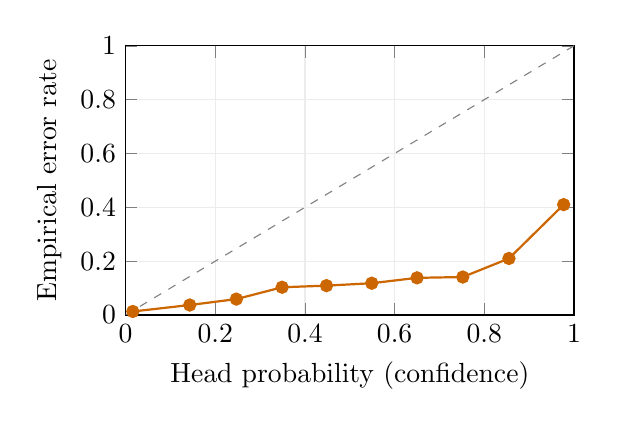
\begin{tikzpicture}
    \begin{axis}[width=0.6\linewidth, height=5.0cm, xlabel={Head probability (confidence)}, ylabel={Empirical error rate},
      xmin=0, xmax=1, ymin=0, ymax=1, grid=major, grid style={gray!15}]
    \addplot[dashed,gray] coordinates {(0,0)(1,1)};
    \addplot[thick,mark=*,color=orange!80!black] coordinates {(0.016,0.013)(0.143,0.037)(0.247,0.059)(0.349,0.103)(0.448,0.109)(0.549,0.118)(0.65,0.138)(0.752,0.141)(0.855,0.21)(0.977,0.41)};
    \end{axis}
  \end{tikzpicture}
  \caption{Reliability of LVH-1.5B. The head is over confident, the curve sits well below the diagonal, so a high score does not mean a high error probability (ECE $=0.238$).}
  \label{fig:calib}
\end{figure}

\section{Case analysis}
\label{app:cases}

We walk through four real ProcessBench cases at 7B, one for each cell of \Cref{fig:agree}. Each box shows the problem and its solution steps, with a mark for whether the generative verifier (\textbf{Gen}) and the introspective head (\textbf{Head}) judge the step correct (\vgood) or an error (\vbad). The step highlighted in the text is the labeled first error. The generative verifier marks a step an error when its value drops below one half; the head marks a step an error when its probability exceeds its 7B operating threshold, about 0.75.

\begin{tcolorbox}[breakable, colback=gray!2, colframe=gray!55, fonttitle=\bfseries\small,
  title={Case 1 (GSM8K). The head catches a fluent but wrong step that generation accepts.}, boxrule=0.5pt, left=2mm, right=2mm, top=1mm, bottom=1mm]
\footnotesize
\textbf{Problem.} It takes James 10 minutes to read 3 pages before bed. He reads 18 pages, then goes to sleep. How long does James spend reading? \emph{(Correct: $18 \div 0.3 = 60$ minutes.)}
\smallskip
\begin{tabularx}{\linewidth}{@{}c X c c@{}}
\toprule
\# & Step & Gen & Head \\
\midrule
1 & Set up: find a reading rate, then use it & \vgood & \vgood \\
2 & Rate $= 3/10 = 0.3$ pages per minute & \vgood & \vgood \\
3 & Total pages read $= 18$ & \vgood & \vgood \\
4 & \textbf{Time $= 18 \times 0.3 = 5.4$ minutes} \; \emph{(first error: needs $\div$, not $\times$)} & \vgood & \vbad \\
5 & Answer: $5.4$ minutes & \vgood & \vbad \\
\bottomrule
\end{tabularx}
\smallskip

\textbf{Gold:} step 4. \quad \textbf{Gen predicts:} none (misses the error). \quad \textbf{Head predicts:} \textbf{step 4 (correct)}.
\smallskip

\textbf{Why.} The two readouts diverge here. The final layer state follows the surface form of the step, and $18 \times 0.3 = 5.4$ is a fluent, locally valid multiplication, so the generated verdict accepts it. The intermediate layer encodes the step against its premises, where the rate is pages per minute and the question asks for minutes, so the correct operation is division; that mismatch is present in the intermediate representation before the surface token is formed, and the residual head reads it out. This is the paper's mechanism in one example, the latent assessment catches a reasoning error that the stated verdict does not.
\end{tcolorbox}

\begin{tcolorbox}[breakable, colback=gray!2, colframe=gray!55, fonttitle=\bfseries\small,
  title={Case 2 (GSM8K). The head avoids a false alarm that generation raises on a correct solution.}, boxrule=0.5pt, left=2mm, right=2mm, top=1mm, bottom=1mm]
\footnotesize
\textbf{Problem.} A two hour concert gives each group 2 minutes on, 6 to perform, 2 off, plus one 10 minute intermission. How many groups can perform? \emph{(Correct: $10n+10\le 120 \Rightarrow 11$ groups; every step is correct.)}
\smallskip
\begin{tabularx}{\linewidth}{@{}c X c c@{}}
\toprule
\# & Step & Gen & Head \\
\midrule
1 & Fit group slots into 120 minutes & \vgood & \vgood \\
2 & Per group $2+6+2 = 10$ minutes \; \emph{(correct)} & \vbad & \vgood \\
3 & Add the 10 minute intermission & \vbad & \vgood \\
4 & Total for $n$ groups is $10n+10$ & \vbad & \vgood \\
5 & Solve $10n+10 \le 120$ & \vbad & \vgood \\
6 & $n \le 11$ & \vbad & \vgood \\
7 & Answer: 11 groups & \vbad & \vgood \\
\bottomrule
\end{tabularx}
\smallskip

\textbf{Gold:} none. \quad \textbf{Gen predicts:} step 2 (false alarm). \quad \textbf{Head predicts:} \textbf{none (correct)}.
\smallskip

\textbf{Why.} The generative verifier reaches its verdict by re-deriving the step, and its own derivation for the per group time disagrees with the solution, so it reports an error where there is none. The head does not re-derive. It reads whether the step is consistent with its premises, and $2+6+2=10$ is, so its error probability stays low on every step. The head is less exposed to this self-inflicted false alarm because it does not run a second, fallible generation. This is the complementary win to Case 1, and the reason the two signals combine well (\Cref{sec:exp-7b}).
\end{tcolorbox}

\begin{tcolorbox}[breakable, colback=gray!2, colframe=gray!55, fonttitle=\bfseries\small,
  title={Case 3 (MATH). Generation localizes an error that the head places one step too early.}, boxrule=0.5pt, left=2mm, right=2mm, top=1mm, bottom=1mm]
\footnotesize
\textbf{Problem.} Let $x>0$ satisfy $x - \tfrac{1}{x} = 3$. Find $x + \tfrac{1}{x}$. \emph{(Correct: $x+\tfrac1x=\sqrt{13}$.)}
\smallskip
\begin{tabularx}{\linewidth}{@{}c X c c@{}}
\toprule
\# & Step & Gen & Head \\
\midrule
1 & $x^2 = 3x + 1$ \; \emph{(correct)} & \vgood & \vbad \\
2 & \textbf{$x^2 - 3x = 1$, factor $(x-1)(x-3)=0$} \; \emph{(first error: wrong factoring)} & \vbad & \vbad \\
3 & $x = 3$, so $x + 1/x = 10/3$ & \vbad & \vbad \\
4 & Answer: $4$ & \vbad & \vbad \\
\bottomrule
\end{tabularx}
\smallskip

\textbf{Gold:} step 2. \quad \textbf{Gen predicts:} \textbf{step 2 (correct)}. \quad \textbf{Head predicts:} step 1 (one step early).
\smallskip

\textbf{Why.} The head localizes to the region of the error but not the exact step. Its per step probability already saturates at step one, the correct setup that leads straight into the bad factoring, so it fires one step early. The intermediate signal is coarse in position, it marks that the derivation is heading wrong, while the fine boundary between the correct setup and the incorrect factoring is exactly what an explicit step by step re-derivation resolves. The generative verifier performs that re-derivation and pins step two. This coarser localization is the price of a single read, and it is why generation still wins the harder localizations at 7B (\Cref{fig:agree}).
\end{tcolorbox}

\begin{tcolorbox}[breakable, colback=gray!2, colframe=gray!55, fonttitle=\bfseries\small,
  title={Case 4 (GSM8K). Both verifiers miss an omission at the first step.}, boxrule=0.5pt, left=2mm, right=2mm, top=1mm, bottom=1mm]
\footnotesize
\textbf{Problem.} In a family of 5, three people eat three eggs each day and the other two eat two each. How many eggs in a week? \emph{(Correct: $(3\cdot3 + 2\cdot2)\cdot7 = 91$.)}
\smallskip
\begin{tabularx}{\linewidth}{@{}c X c c@{}}
\toprule
\# & Step & Gen & Head \\
\midrule
1 & \textbf{Count $3$ people $\times 3$ eggs, then $\times 7$ days} \; \emph{(first error: omits the other 2 people)} & \vgood & \vgood \\
2 & $9$ eggs/day $\times 7 = 63$ & \vbad & \vgood \\
3 & $63$ eggs & \vbad & \vbad \\
\bottomrule
\end{tabularx}
\smallskip

\textbf{Gold:} step 1. \quad \textbf{Gen predicts:} step 2 (wrong). \quad \textbf{Head predicts:} step 3 (wrong).
\smallskip

\textbf{Why.} The error is one of omission, not of a wrong statement. Step one, count three people times three eggs, is true as far as it goes; what is wrong is the missing contribution of the other two people, which never appears as a locally incorrect step. Both verifiers score each step against its premises, and a step that is locally valid but incomplete passes either test, so both drift to a later step. Errors of omission are a property of the whole solution rather than of one step, so a step local read, generative or introspective, shares this blind spot. These are the 67 both wrong cases of \Cref{fig:agree}, and they mark where step level verification itself, not the choice of reading it, reaches its limit.
\end{tcolorbox}
